\section{Theoretical AGN-Host Colour Space Results}
\subsection{SWIRE}
By introducing Type 1 and Type 2 AGN into our composite, we can see how AGN can potentially affect a galaxies' colours. An initial set of composites were created using the SWIRE template library. Figure \ref{fig:subplots} presents the UVJ colour evolution for both the Type 1 and Type 2 composite galaxies.
\begin{figure}[h!]
    \centering
    \begin{subfigure}[b]{0.45\textwidth}   
  % Align at the bottom
        \centering
        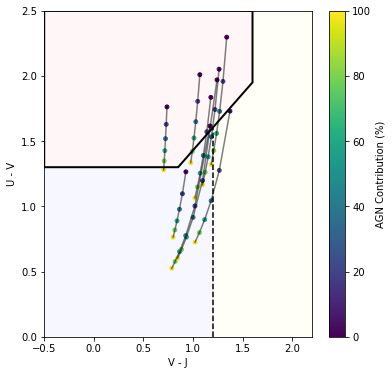
\includegraphics[width=\textwidth]{Images/TheoreticalModelPlots/SWIREType1AGNUVJ.png}
    \end{subfigure}
    \hfill
    \begin{subfigure}[b]{0.45\textwidth}  % Align at the bottom
        \centering
        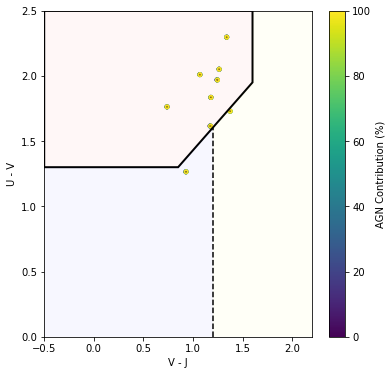
\includegraphics[width=\textwidth]{Images/TheoreticalModelPlots/SWIREType2AGNUVJ.png}
    \end{subfigure}
    \caption{UVJ colour evolution for a Type 1 (left) and Type 2 (right) AGN composite using a subset of the SWIRE galaxy template set. Lighter colours reflect a higher AGN contribution added with the colour evolution path connected with a line.}
    \label{fig:subplots}
\end{figure}\\
In these plots, we see a change in UVJ position with increasing AGN contribution for the Type 1 AGN composites, while the Type 2 AGN composite does not seem to show any discernible movement within the UVJ colour space. Further theoretical colour modelling was tested using the GALSEDATLAS templates to test if this result was reproducible using a larger set of galaxy templates.
\newpage
\subsection{GALSEDATLAS}
\subsubsection{UVJ Results}
Figure \ref{fig:Brown-Type1Composite_UVJ} illustrates the UVJ colour evolution of a Type 1 AGN composite as the AGN contribution increases. The corresponding galaxy fractions for each region are indicated in the corner of the plot (see Appendix A for detailed tables). The initial value of $\alpha = 0$\% shows the galaxy without any AGN present. We observe a clear trend of sources moving toward the star-forming region of the UVJ diagram, similar to Figure \ref{fig:subplots}. The final plot within this figure overlays all sources onto a heat map showing where AGN may cause galaxies to end up within the UVJ diagram, showing a concentration of galaxies along the diagonal of the UVJ diagram, with the majority of sources being located at V- J $>$ 0.5 within the star-forming region. The galaxy population fraction is located in each region of the UVJ diagram and corresponds to the fraction of galaxies from all sources within a particular region. We see in the theoretical model that there is a higher fraction of quiescent galaxies within the UVJ diagram at low alpha values. However, as the AGN contribution increases, the quiescent fraction drops. In contrast, the dusty fraction slightly increases, and the star-forming fraction drastically increases.
\begin{figure}[h!]
    \centering
    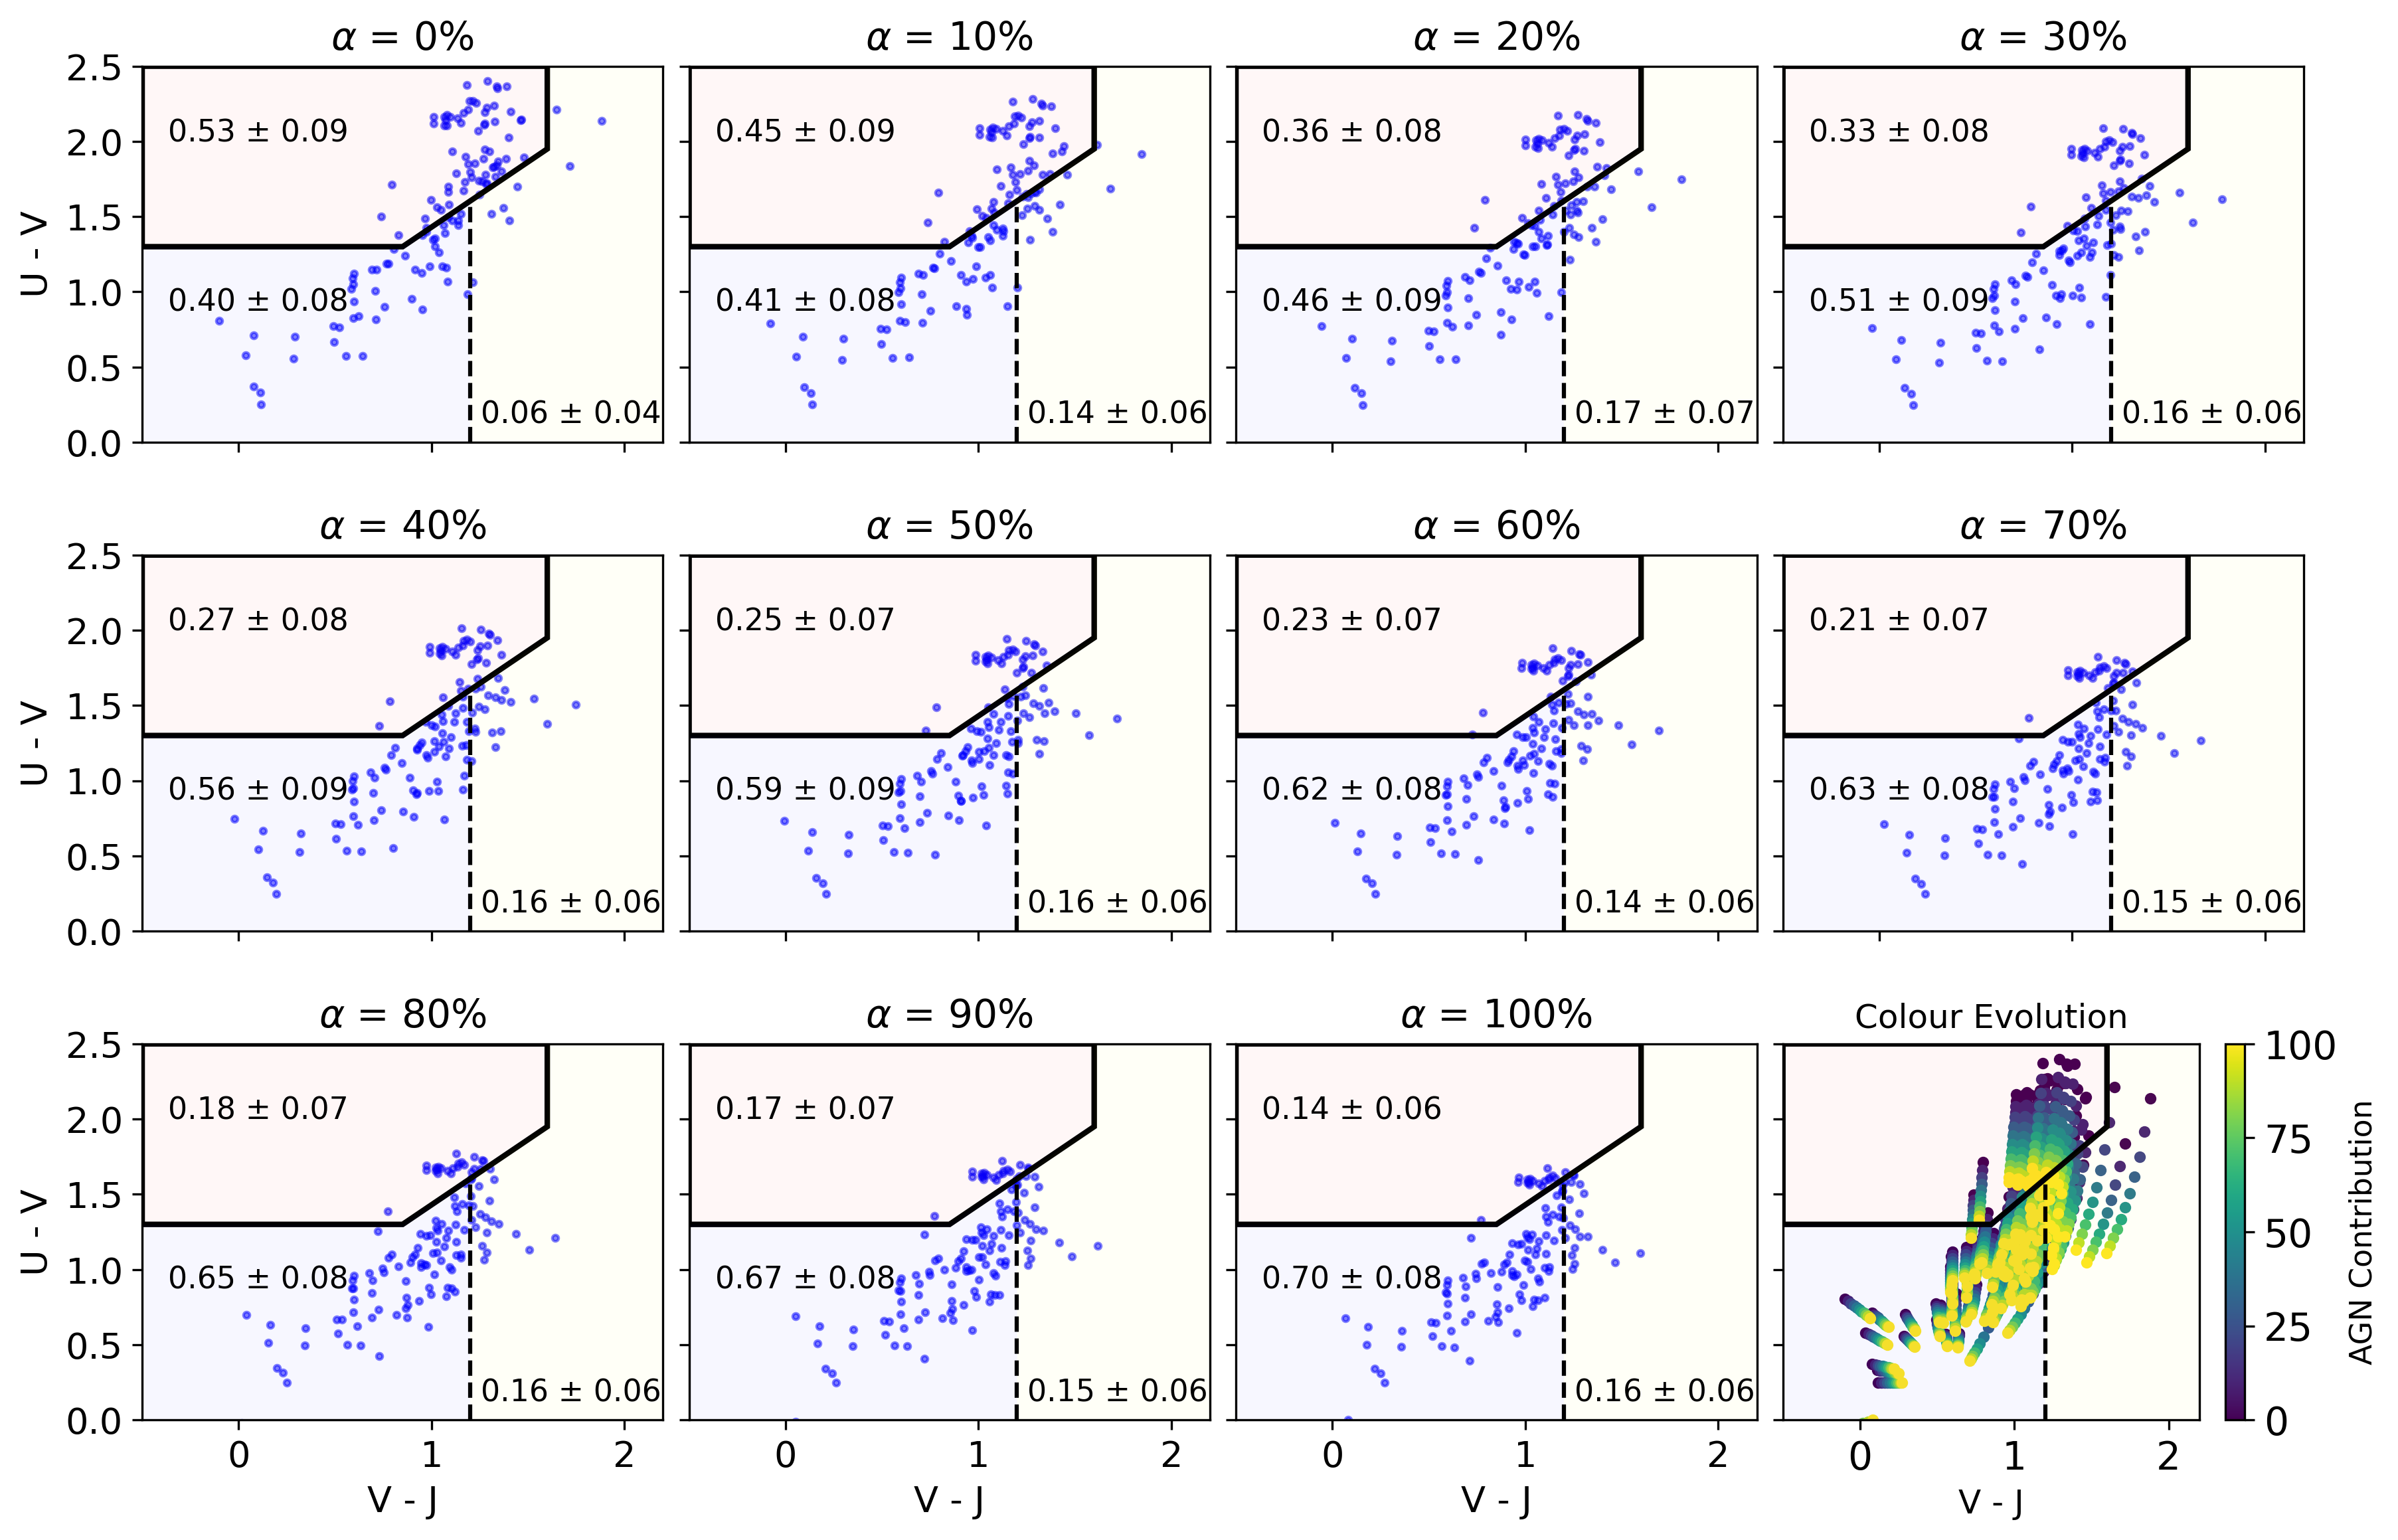
\includegraphics[width=1\linewidth]{Images/TheoreticalModelPlots/UVJ_evolution_Type1AGN_Brown.png}
    \caption{The colour evolution in the UVJ diagram for a Type 1 AGN composite SED constructed using the GALSEDATLAS templates. This template set allows for more galaxy composites to be modelled than the SWIRE set. The plot above shows the fraction of the population belonging to each region within their respective regions.}
    \label{fig:Brown-Type1Composite_UVJ}
\end{figure} \\
We can see that increasing the AGN contribution within these models has a minimal impact on the UVJ position of the sources. Additionally, incorporating a Type 2 AGN contribution yields no substantial change in the overall galaxy fractions of the composites, except for a minor reduction in the quiescent fraction accompanied by a corresponding 1\% increase in the dusty fraction. 
\begin{figure}[ht]
    \centering
    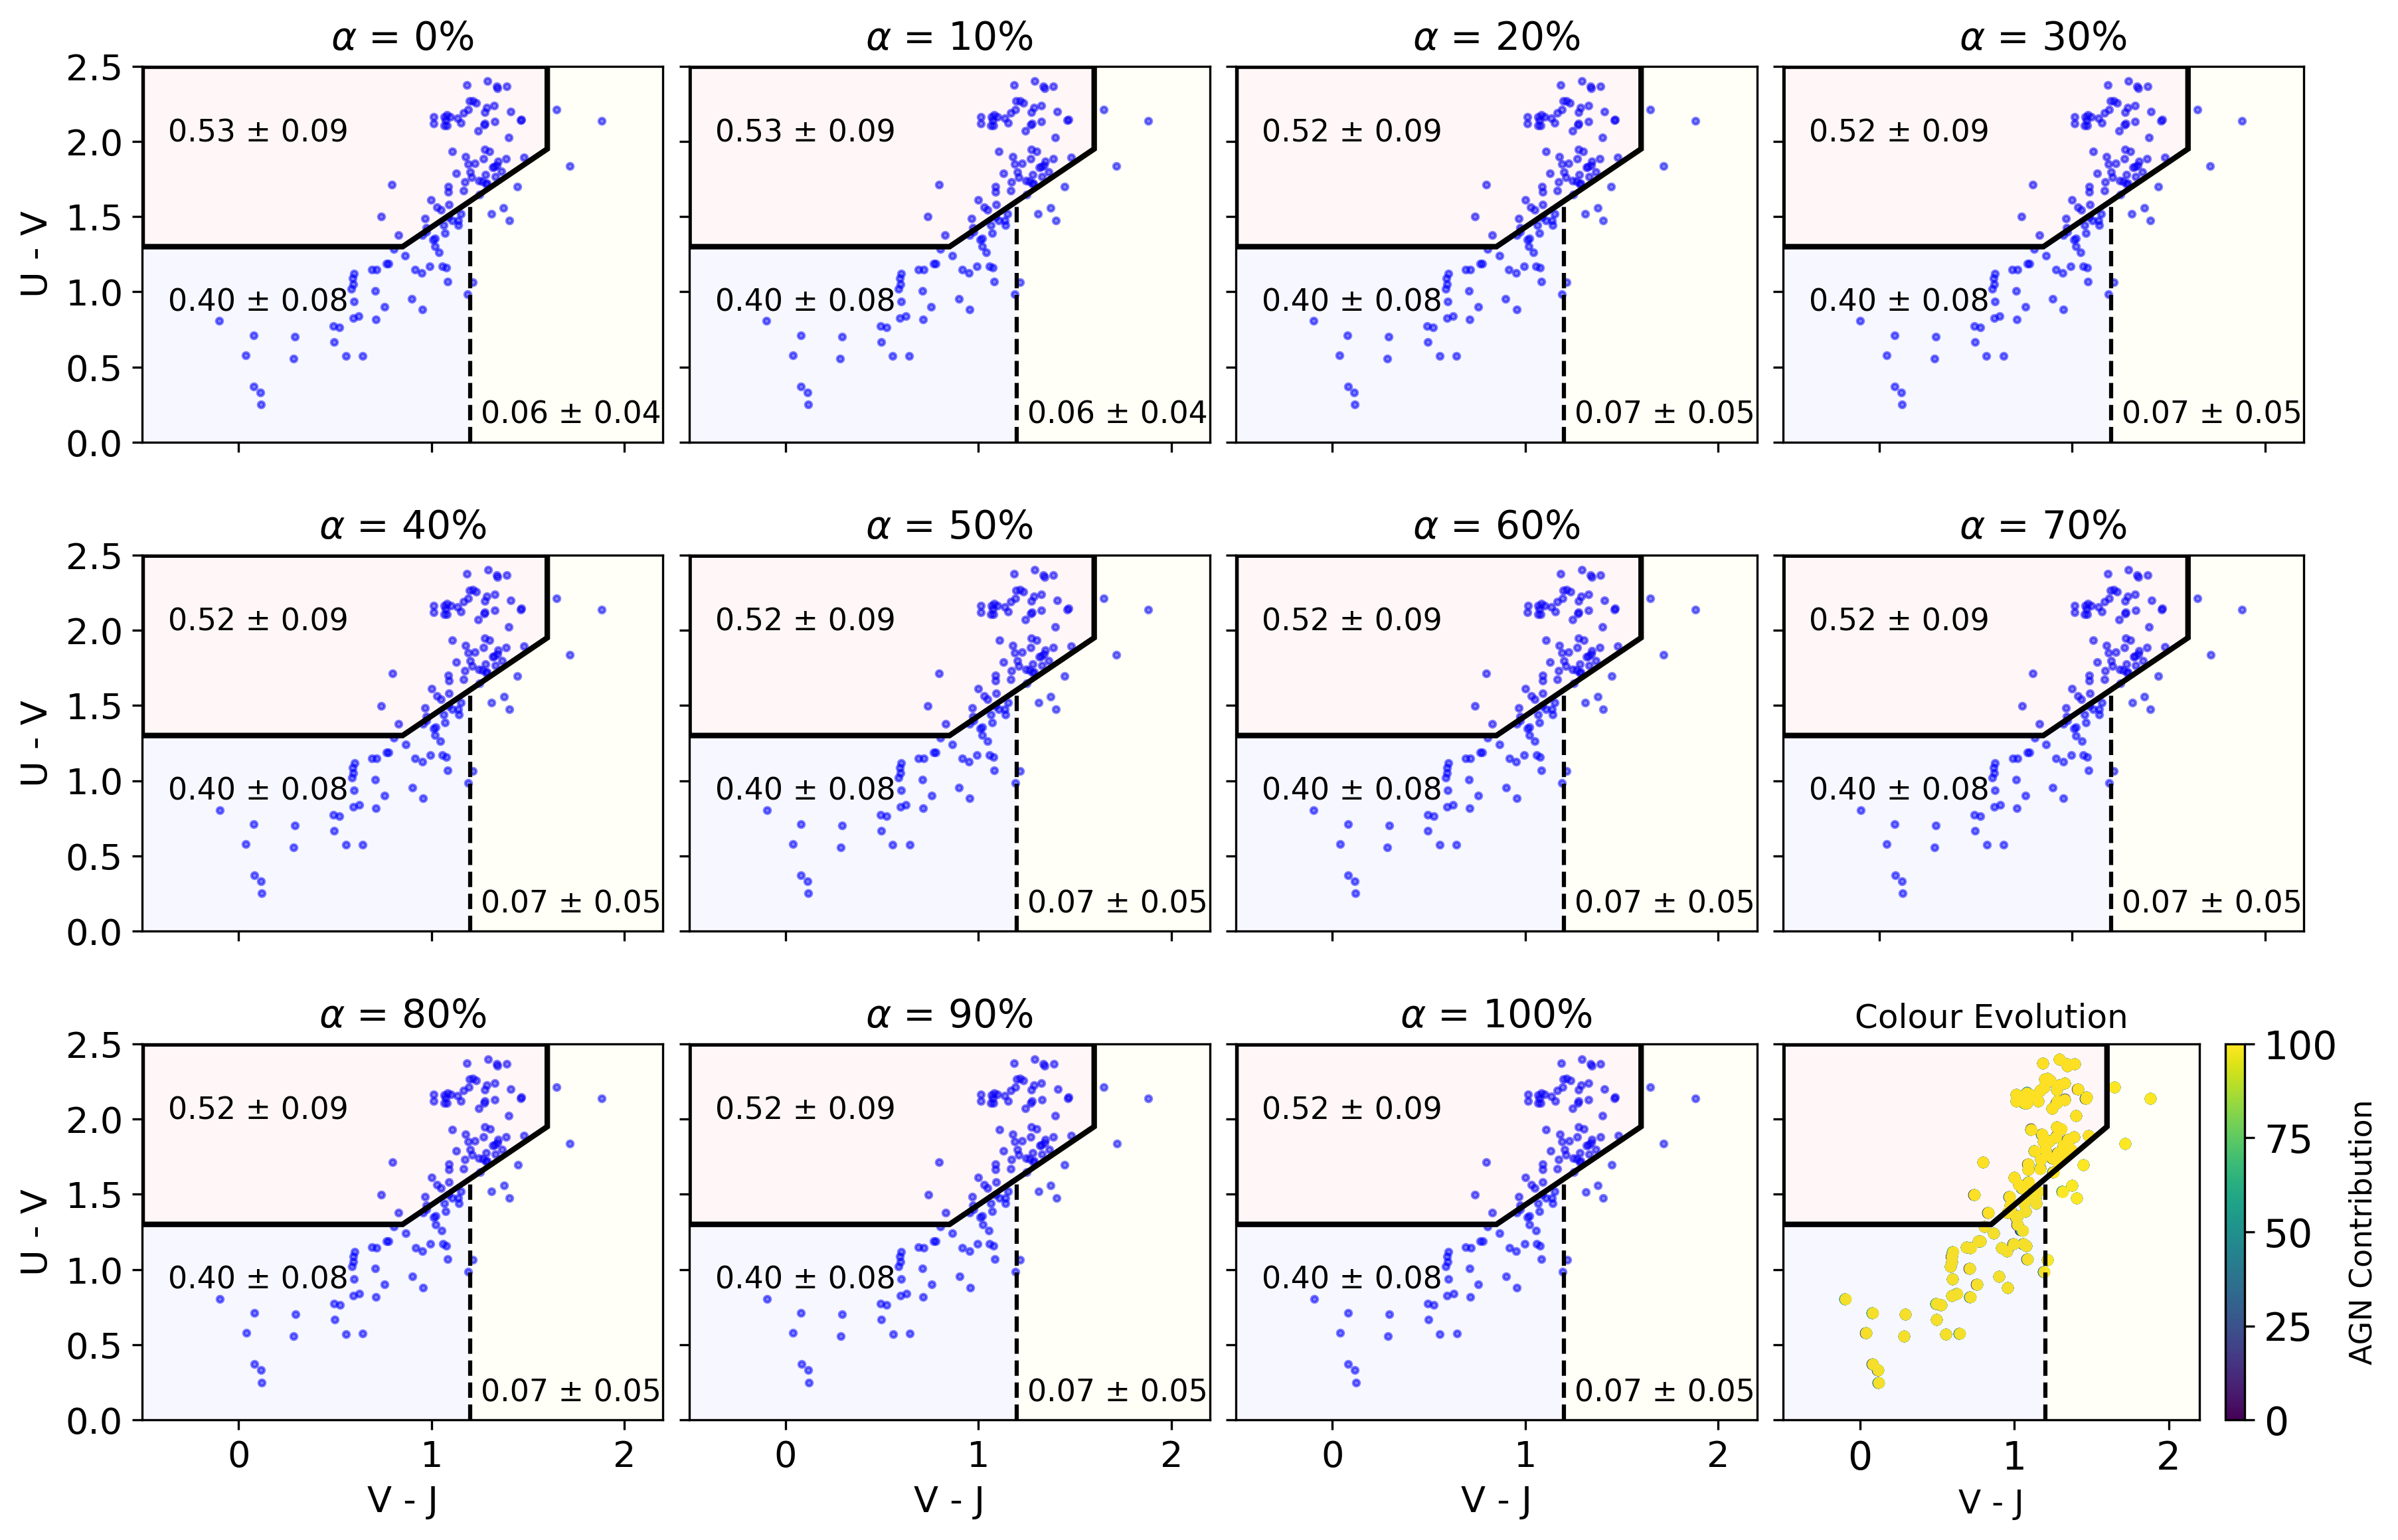
\includegraphics[width=1\linewidth]{Images/TheoreticalModelPlots/UVJ_evolution_Type2AGN_Brown.png}
    \caption{The colour evolution in the UVJ diagram for a Type 2 AGN composite SED constructed using the GALSEDATLAS templates.}
    \label{fig:Brown-Type2Composite_UVJ}
\end{figure} \\ To quantify the change in position for each composite type, we calculated the average position for all positions within the UVJ diagram at each alpha value. A vector offset was then used to measure the movement from the initial position with increasing AGN contribution. As shown in Table \ref{tab:UVJ_vectoroffset}. For Type 1 AGN composites, a 10\% AGN contribution shifted the average UVJ position by 0.08 dex while increasing the AGN contribution to 100\% caused the average movement to be increased to 0.47 dex. In contrast, Type 2 composites exhibited no discernible change in their average UVJ position. \\
% It'll be useful to put that table here to show the movement
\begin{table}[h!]
    \centering
    \begin{tabular}{llllllllllll} 
        \hline
        \textbf{AGN Contribution (\%)} & \textbf{10} & \textbf{20} & \textbf{30} & \textbf{40} & \textbf{50} & \textbf{60} & \textbf{70} & \textbf{80} & \textbf{90} & \textbf{100} \\ \hline
        \textbf{Type 1 Composite} & 0.08 & 0.15 & 0.20 & 0.25 & 0.30 & 0.34 & 0.38 & 0.41 & 0.44 & 0.47 \\
        \textbf{Type 2 Composite} & 0.00 & 0.00 & 0.00 & 0.00 & 0.00 & 0.00 & 0.00 & 0.00 & 0.00 & 0.00 \\ 
        \hline
    \end{tabular}
    \caption{Mean Vector Offsets from the initial position for Different AGN Composite Model Types and AGN Contribution amounts in the UVJ rest frame colour space}
    \label{tab:UVJ_vectoroffset}
\end{table} \\
These findings mirror the trends observed in the SWIRE composites as shown in Figure \ref{fig:subplots}. Ultimately, Type 1 AGN composites exhibit a characteristic shift towards the star-forming region with increasing AGN contribution. In contrast, Type 2 AGN composites remain largely stationary in the UVJ diagram at all AGN contributions. Consequently, Type 1 composites increase the star-forming fraction while decreasing galaxies' quiescent and dusty fractions. Type 2 composites, on the other hand, don't appear to impact the overall galaxy fraction distribution. 
\newpage
\subsubsection{ugr Results}
The ugr diagram in Figure \ref{fig:Brown-Type1Composite_ugr} illustrates the colour evolution of Type 1 composites on the ugr colourspace. The completeness of the selection is indicated in the corner of the selection region (See Appendix A for detailed tables). In these diagrams, a colour selection wedge aims to identify galaxies within the redshift range of $2.6 < z < 3.6$. These target galaxies are coloured yellow to visually assess the effectiveness of the selection. In the text on the top left panel, we see the fraction of correct selections of all selections, corresponding to the completeness value. As we increase the AGN contribution for these models, we see that all sources within this diagram migrate towards a point around (0, 0) in the ugr diagram. As AGN contribution increases in the models, we observe a migration of all sources towards the point (0, 0) in the ugr diagram. In particular, yellow (target redshift) and cyan (high redshift) sources exhibit significant movement. This leads to a sharp decline in completeness, dropping from 0.67 to 0.17 with only a 10\% AGN contribution. The completeness reaches 0 at 70\% AGN contribution, after which the points appear to stabilize. The plot in the bottom right panel of Figure \ref{fig:Brown-Type1Composite_ugr} visualises the colour evolution of the composites with increasing AGN contribution. It reveals a distinct locus below the selection region, indicating where these composites cluster in the colourspace.
\begin{figure}[h!]
    \centering
    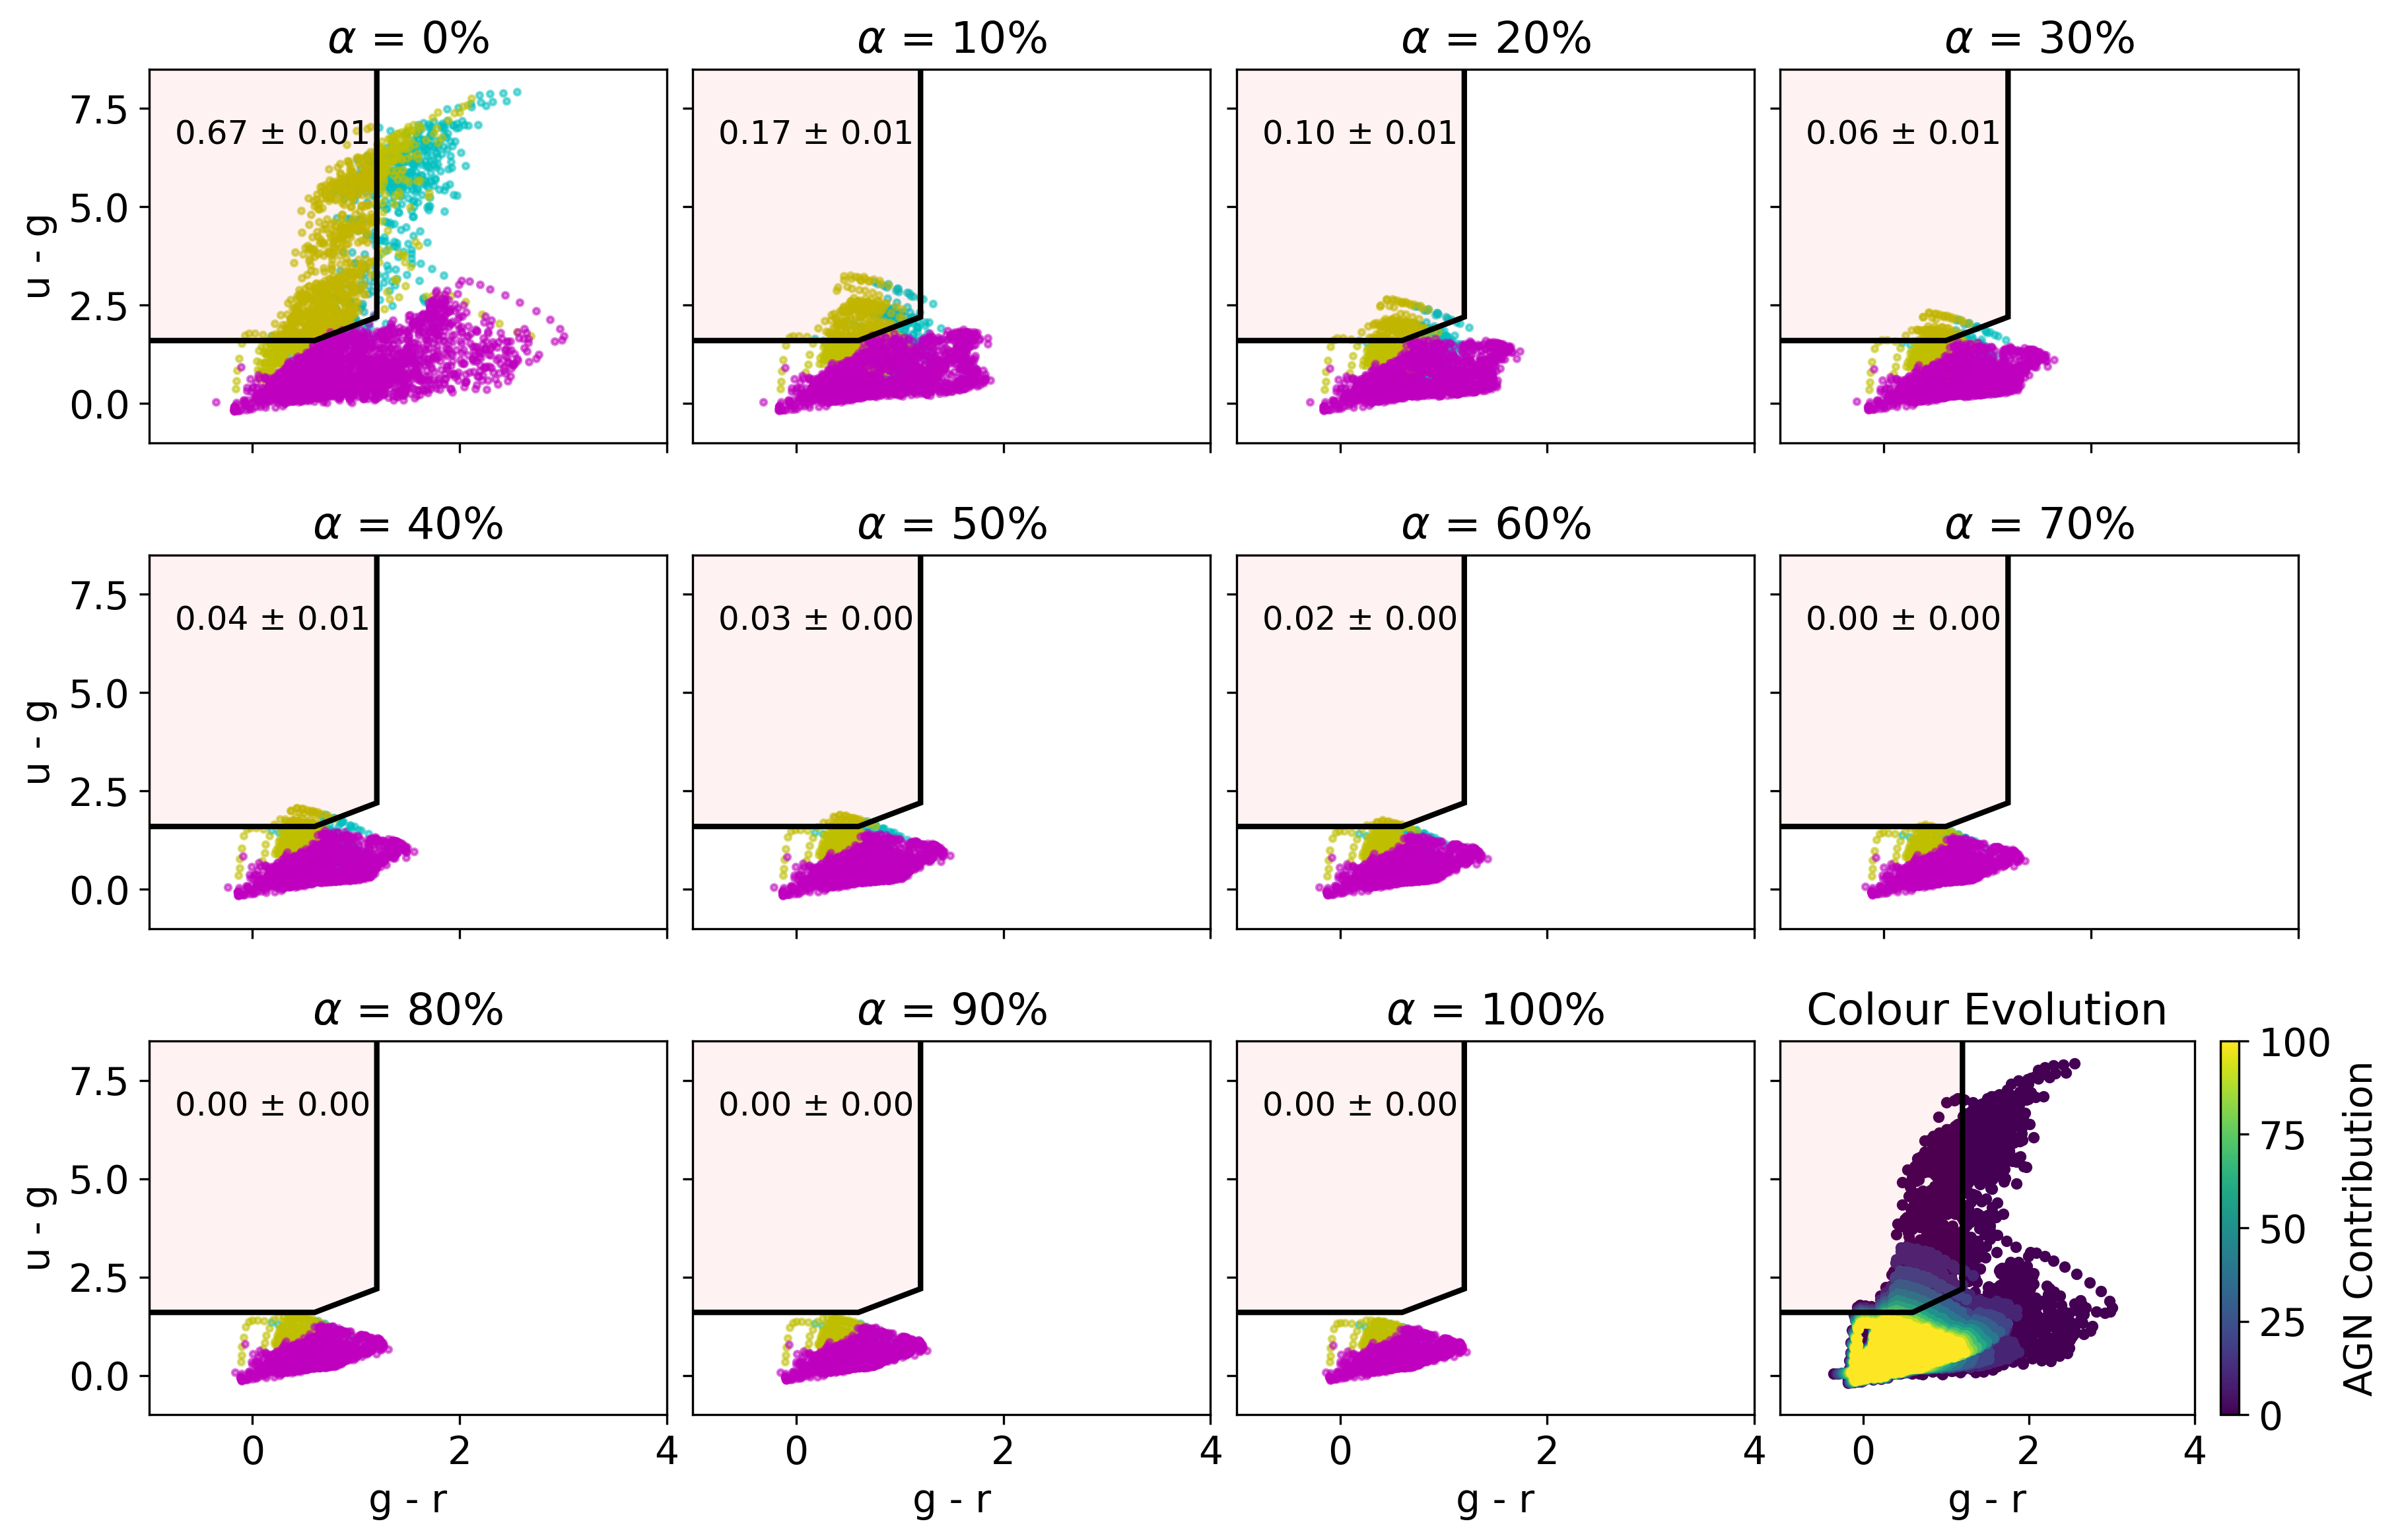
\includegraphics[width=1\linewidth]{Images/TheoreticalModelPlots/ugr_evolution_Type1AGN_Brown.png}
    \caption{The colour evolution in the ugr diagram for a Type 1 AGN composite SED constructed using the GALSEDATLAS templates. Galaxies within a redshift range of 2.6 $<$ z $<$ 3.6 are shown in yellow, galaxies with a redshift greater than 3.6 are shown in cyan, and redshifts less than 2.6 are shown in magenta.}
    \label{fig:Brown-Type1Composite_ugr}
\end{figure}\\
Unlike Type 1 AGN composites, Type 2 AGN composites exhibit minimal change to the ugr colourspace (See Figure \ref{fig:Brown-Type2Composite_ugr}). Contrary to Type 1 AGN Composites, increasing AGN contribution does not lead to a noticeable migration of all sources within the diagram. Only sources with a redshift greater than 3.6 appear affected, resulting in no significant drop in completeness with increasing AGN contribution. The colour evolution in the bottom right panel shows no distinct clustering or locus of composites below the selection region, suggesting minimal colour evolution with varying AGN contribution.
\begin{figure}[h!]
    \centering
    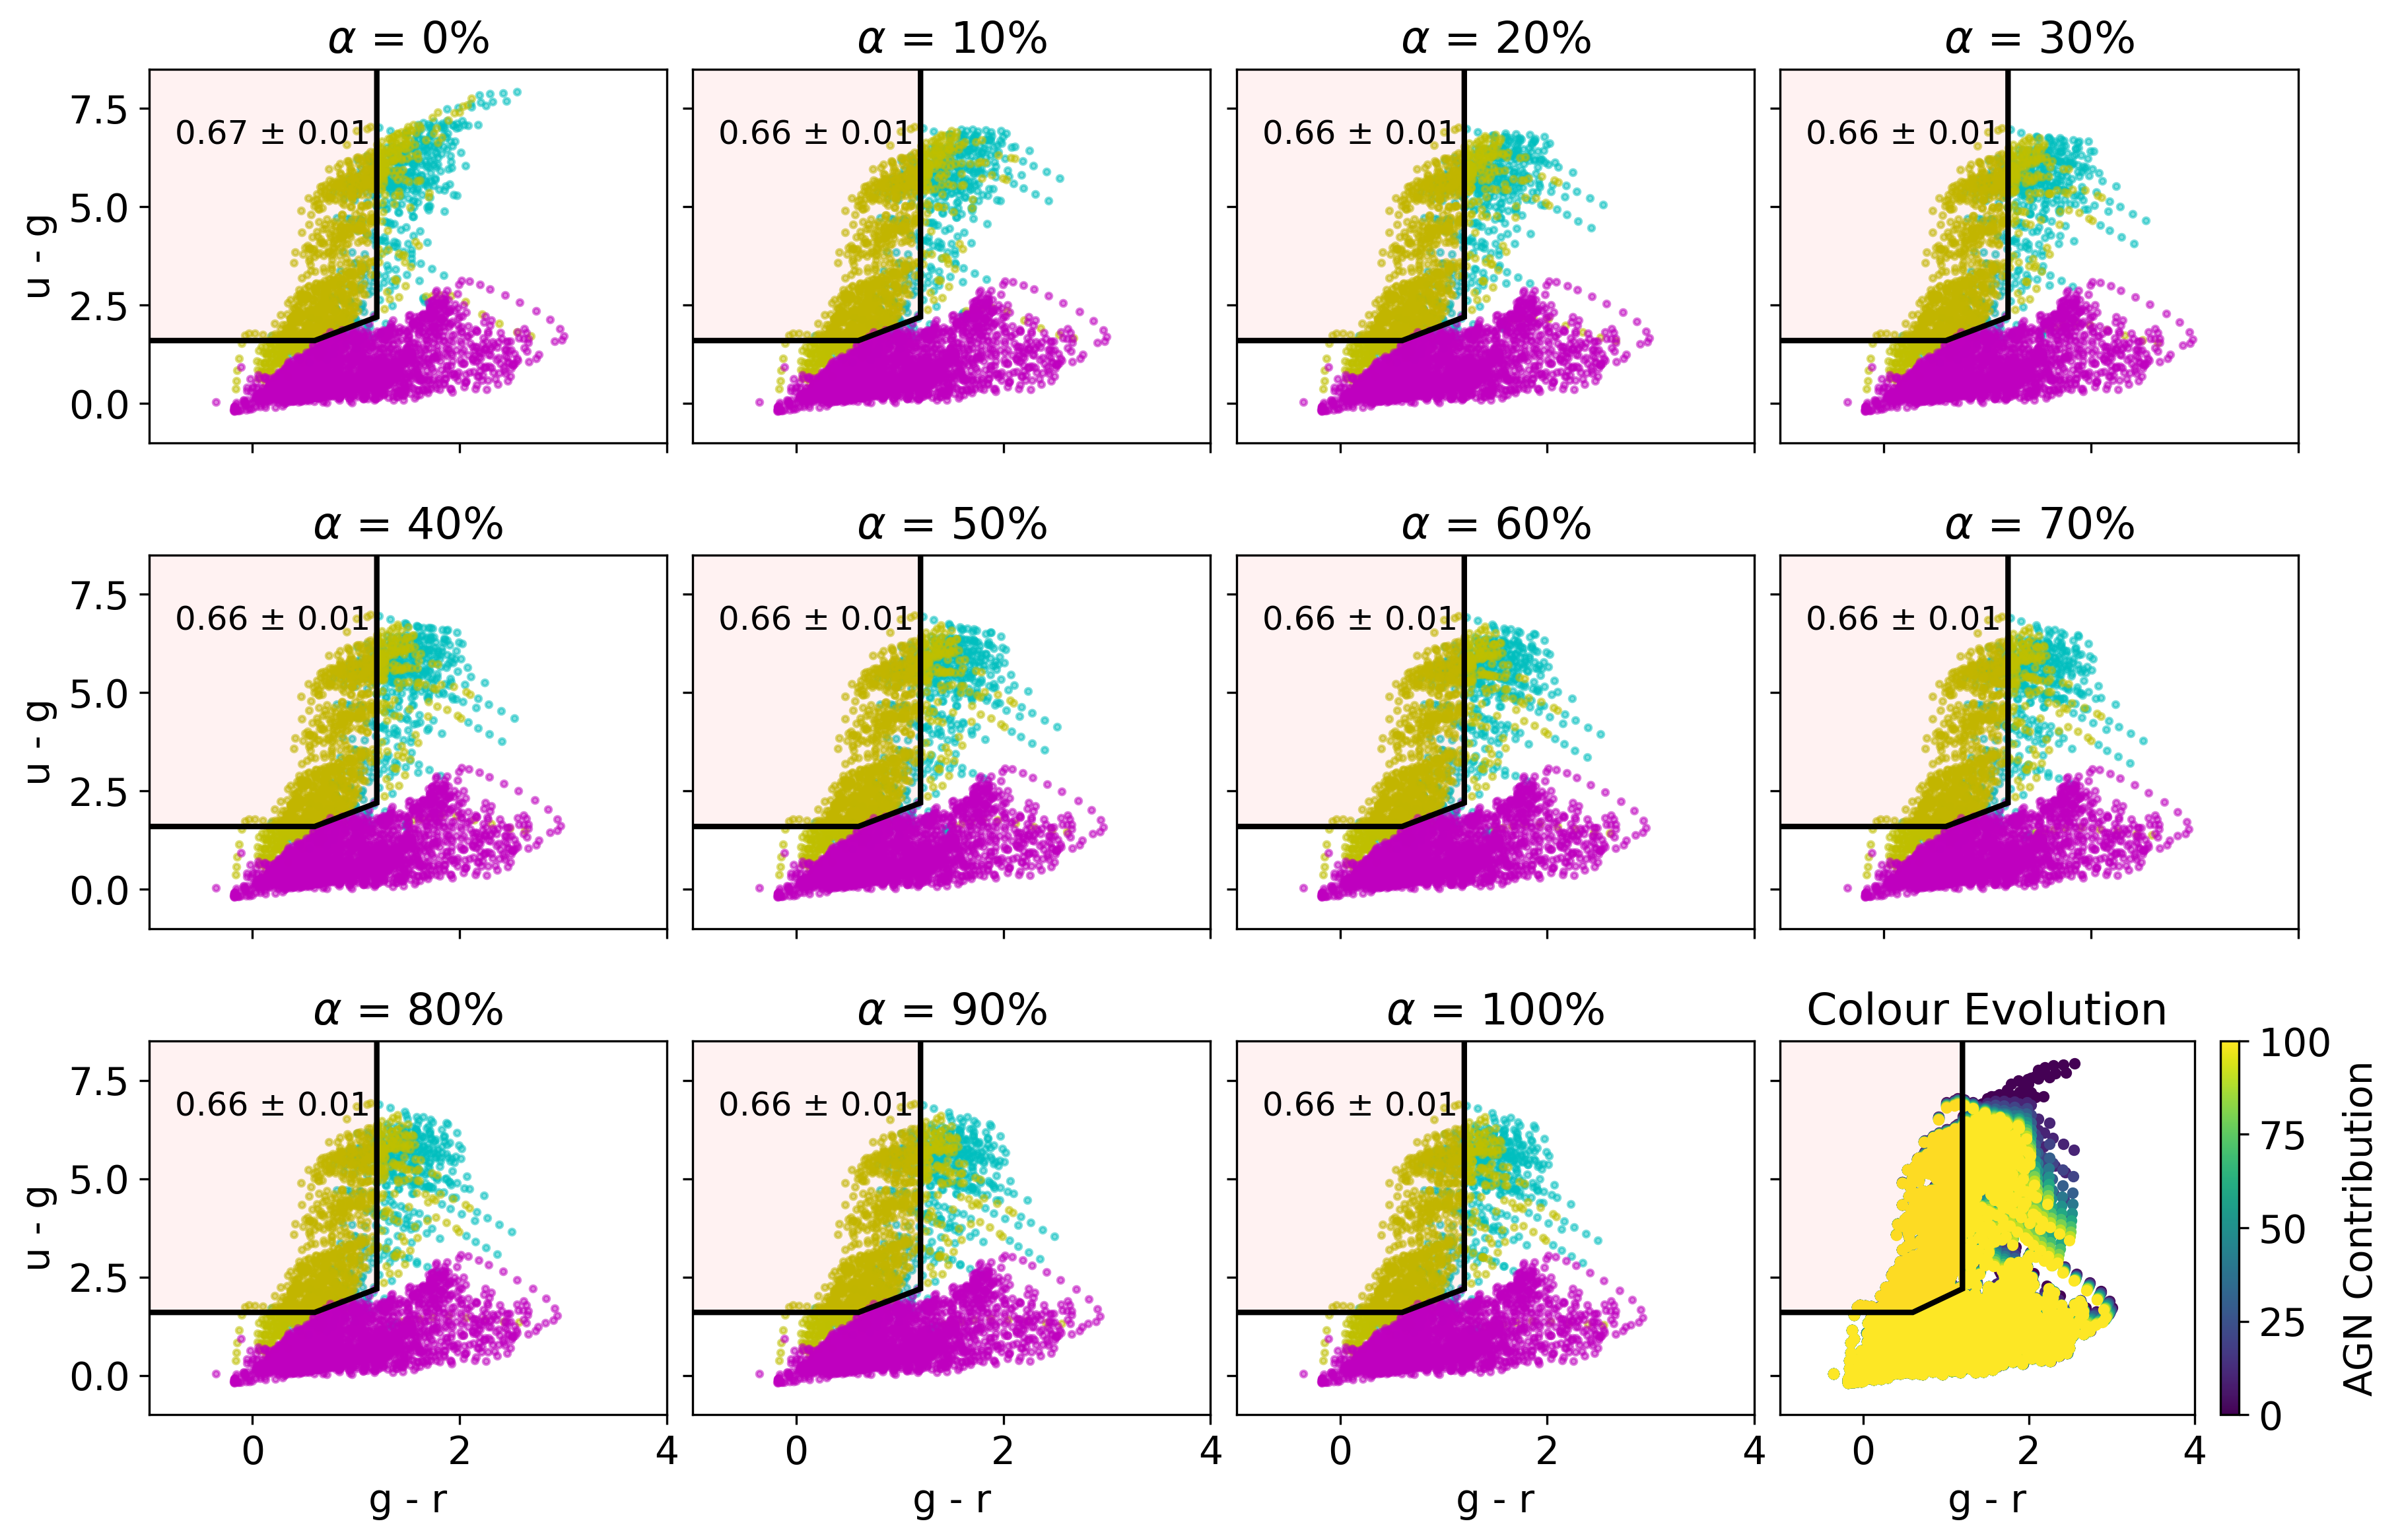
\includegraphics[width=1\linewidth]{Images/TheoreticalModelPlots/ugr_evolution_Type2AGN_Brown.png}
    \caption{The colour evolution in the ugr diagram for a Type 2 AGN composite SED constructed using the GALSEDATLAS templates}
    \label{fig:Brown-Type2Composite_ugr}
\end{figure} \\
Table \ref{tab:ugr_vectoroffset} shows the mean vector offset from the initial position for Type 1 and Type 2 AGN composites across varying AGN contribution levels in the ugr colour space. As AGN contribution increases from 10\% to 100\%, Type 1 composites exhibit a substantial shift in their average position, with the mean vector offset of 1.11 dex at just 10\% contribution, increasing to 1.52 dex at 100\% contribution. In contrast, Type 2 composites show minimal change, with the offset rising only slightly from 0.02 to 0.08, indicating relative stability in their position despite increasing AGN influence. \\
\begin{table}[h!]
    \centering
    \begin{tabular}{llllllllllll} 
        \hline
        \textbf{AGN Contribution (\%)} & \textbf{10} & \textbf{20} & \textbf{30} & \textbf{40} & \textbf{50} & \textbf{60} & \textbf{70} & \textbf{80} & \textbf{90} & \textbf{100} \\ \hline
        \textbf{Type 1 Composite} & 1.11 & 1.25 & 1.33 & 1.38 & 1.42 & 1.45 & 1.47 & 1.49 & 1.51 & 1.52 \\
        \textbf{Type 2 Composite} & 0.02 & 0.03 & 0.04 & 0.05 & 0.05 & 0.06 & 0.07 & 0.07 & 0.08 & 0.08 \\ 
        \hline
    \end{tabular}
    \caption{Mean Vector Offsets from the initial position for Different AGN Composite Model Types and AGN Contribution amounts in the ugr colour space}
    \label{tab:ugr_vectoroffset}
\end{table} \\
There is a noticeable difference in the colour evolution of Type 1 and Type 2 AGN composites. The dramatic shift and clustering in Type 1 composites cause the selection wedge to fail even at low AGN contribution levels, significantly impacting completeness. In contrast, Type 2 composites have only a minor effect on the ugr colourspace and do not affect completeness. This distinction is visually reinforced by the colour evolution plot, which shows a pronounced locus below the selection region exclusively for Type 1 composites, highlighting the difference in colour evolution in response to AGN contribution.
\subsubsection{IRAC Results}
The lacy wedge used in the IRAC colour space is useful for selecting AGN from a sample where the AGN is unknown; this colour space is most useful for Type 2 AGN where MIR reprocessing of light causes a characteristic IR colour. In Figure \ref{fig:Brown-Type1Composite_IRAC} the effect of Type 1 AGN composites on the IR colour space are explored, additionally the completeness is included in the selection region (See Appendix A for details). By increasing AGN contribution, galaxies systematically move outside of the selection region. This is reflected in the completeness value, which is reduced from 0.26 to 0.06 as the AGN contribution increases from 0\% to 100\%. The AGN colour evolution plot displays a clear clustering outside the selection region for large AGN contribution amounts.
\begin{figure}[h!]
    \centering
    
\includegraphics[width=1\linewidth]{Images/TheoreticalModelPlots/IRAC_evolution_Type1AGN_Brown.png}
    \caption{The colour evolution in the IRAC diagram for a Type 1 AGN composite SED constructed using the GALSEDATLAS templates. Only restframe galaxies are included in this plot due to the way the galaxies were artificially redshifted. }
    \label{fig:Brown-Type1Composite_IRAC}
\end{figure}
\\While the IRAC diagram shows a clear removal of sources from the selection region for Type 1 AGN composites, Type 2 composites are shown to have the opposite effect (See Figure \ref{fig:Brown-Type2Composite_IRAC}). This figure illustrates that increasing the AGN contribution in these composites leads to a dramatic rise in the completeness of the selection wedge, bringing a substantial number of sources into the selection region. With an AGN contribution of 70\%, over 98\% of sources fall within this region. The heat-map further confirms this trend, showcasing a distinct clustering within the selection region for AGN contributions of 30\% or higher. \\Table \ref{tab:irac_vectoroffset} shows the mean displacement for each composite set. We see that, unlike the UVJ and ugr colour spaces, there is an apparent increase in displacement for both Type 1 and Type 2 AGN composites across all AGN contributions, Notably, this increase is more pronounced in Type 2 composites compared to Type 1. At 100\% AGN contribution, the displacement can reach as high as 0.18 dex for Type 1 and 0.25 dex for Type 2 composites. \\\\While Type 1 AGN composites noticeably impact UVJ and ugr colour space, Type 2 AGN are shown to have little effect. In contrast, both AGN types were shown to significantly alter the IRAC colour space. Type 1 AGN reduces completeness by pushing sources outside the selection region, while Type 2 AGN increases completeness by clustering them. This contrast is vividly illustrated in the AGN contribution colour evolution plot for the IRAC colour space (Figures \ref{fig:Brown-Type1Composite_IRAC} and \ref{fig:Brown-Type2Composite_IRAC}, bottom left panels).
\begin{figure}[h!]
    \centering
    
\includegraphics[width=1\linewidth]{Images/TheoreticalModelPlots/IRAC_evolution_Type2AGN_Brown.png}
    \caption{The colour evolution in the IRAC diagram for a Type 1 AGN composite SED constructed using the GALSEDATLAS templates}
    \label{fig:Brown-Type2Composite_IRAC}
\end{figure}
\begin{table}[h!]
    \centering
    \begin{tabular}{llllllllllll} 
        \hline
        \textbf{AGN Contribution (\%)} & \textbf{10} & \textbf{20} & \textbf{30} & \textbf{40} & \textbf{50} & \textbf{60} & \textbf{70} & \textbf{80} & \textbf{90} & \textbf{100} \\ \hline
        \textbf{Type 1 Composite} & 0.04 & 0.06 & 0.08 & 0.10 & 0.12 & 0.13 & 0.15 & 0.16 & 0.17 & 0.18 \\
        \textbf{Type 2 Composite} & 0.06 & 0.10 & 0.13 & 0.15 & 0.17 & 0.19 & 0.21 & 0.22 & 0.24 & 0.25 \\ 
        \hline
    \end{tabular}
    \caption{Mean Vector Offsets from the initial position for both AGN Composite Model Types and AGN Contribution amounts for IRAC composites.)}
    \label{tab:irac_vectoroffset}
\end{table}
\newpage
